\documentclass[11pt,a4paper]{report}

\usepackage[utf8]{inputenc}
\usepackage[T1]{fontenc}
\usepackage[italian]{babel}
\usepackage{lmodern}
\usepackage[margin=2.6cm]{geometry}
\usepackage{graphicx}
\usepackage{booktabs}
\usepackage{siunitx}
\usepackage{caption}
\usepackage{xcolor}
\usepackage{microtype}
\usepackage[hidelinks]{hyperref}
\usepackage{float}
\usepackage{tabularx}

\captionsetup{font=small,labelfont=bf,width=0.92\textwidth}
\sisetup{output-decimal-marker={,},group-separator={.},group-minimum-digits=4}
\setlength{\parskip}{0.4em}
\setlength{\parindent}{0pt}
\renewcommand{\arraystretch}{1.25}

\definecolor{autoblue}{HTML}{1f5fa8}
\definecolor{partgold}{HTML}{c99a12}
\definecolor{judgegray}{HTML}{6f747b}

\begin{document}

\chapter{La frontiera dell'automazione nel Molecular Tumor Board}
\label{ch:frontiera-automazione}

\section{La domanda}

I capitoli precedenti hanno misurato \emph{quanto bene} un sistema GraphRAG
risponde a domande di oncologia di precisione rispetto a un RAG testuale. Ma
il risultato che conta davvero per la pratica clinica è un altro, e più
ambizioso: \textbf{quanta parte del lavoro di preparazione di un Molecular
Tumor Board (MTB) può essere realisticamente automatizzata, e quale parte
resta intrinsecamente nel dominio del giudizio multidisciplinare?}

La tesi che sostengo in questo capitolo è che la risposta non va
\emph{ipotizzata}: i quattro esperimenti condotti (accuratezza multi-hop,
generalizzabilità tra reader, robustezza alla riformulazione, sicurezza e
astensione) la \emph{misurano} già. Messi insieme, tracciano
empiricamente una ``frontiera dell'automazione'' che attraversa il workflow
MTB in un punto preciso.

\section{Il workflow MTB, decomposto}

La preparazione di un Molecular Tumor Board non è un'operazione monolitica:
è una catena di stadi con nature epistemiche molto diverse. Alcuni stadi
sono \emph{recuperi di fatti} --- cercare, collegare e verificare
informazioni già esistenti in banche dati curate. Altri sono
\emph{ponderazioni di giudizio} --- pesare evidenze contrastanti,
contestualizzare al singolo paziente, assumersi la responsabilità di una
raccomandazione. Se si scompone il workflow in questi stadi, i risultati
sperimentali si collocano in modo netto su ciascuno di essi
(Tabella~\ref{tab:stadi}, Figura~\ref{fig:frontiera}).

\begin{table}[H]
\centering
\caption{I dieci stadi della preparazione MTB, classificati per grado di
automatizzabilità sulla base dei risultati sperimentali. La ``frontiera''
passa tra lo stadio 5 e lo stadio 6.}
\label{tab:stadi}
\small
\begin{tabularx}{\textwidth}{c X l}
\toprule
\# & Stadio della preparazione MTB & Natura \\
\midrule
\multicolumn{3}{l}{\textcolor{autoblue}{\textbf{Automatizzabile --- validato sperimentalmente}}}\\
1 & Annotazione varianti (gene, tipo, HGVS/dbSNP) & look-up strutturato \\
2 & Assemblaggio catene variante$\to$gene$\to$farmaco$\to$evidenza$\to$trial & cross-referencing multi-hop \\
3 & Recupero companion diagnostics / approvazioni FDA & look-up relazionale \\
\midrule
\multicolumn{3}{l}{\textcolor{partgold}{\textbf{Parzialmente automatizzabile --- assistivo}}}\\
4 & Pre-screening eleggibilità trial (criteri strutturati) & matching su criteri \\
5 & Armonizzazione livelli di evidenza (CIViC A--E vs OncoKB) & normalizzazione semantica \\
\midrule
\multicolumn{3}{l}{\textcolor{judgegray}{\textbf{Intrinsecamente giudizio multidisciplinare}}}\\
6 & Ponderazione di evidenze deboli o contrastanti & giudizio \\
7 & Integrazione del contesto-paziente (comorbidità, linee, PS, organi) & giudizio clinico \\
8 & Priorità tra alterazioni multiple azionabili & giudizio multidisciplinare \\
9 & Off-label / uso compassionevole, etica, accesso, costi & giudizio + responsabilità \\
10 & Raccomandazione terapeutica finale e accountability & responsabilità legale \\
\bottomrule
\end{tabularx}
\end{table}

\begin{figure}[H]
\centering
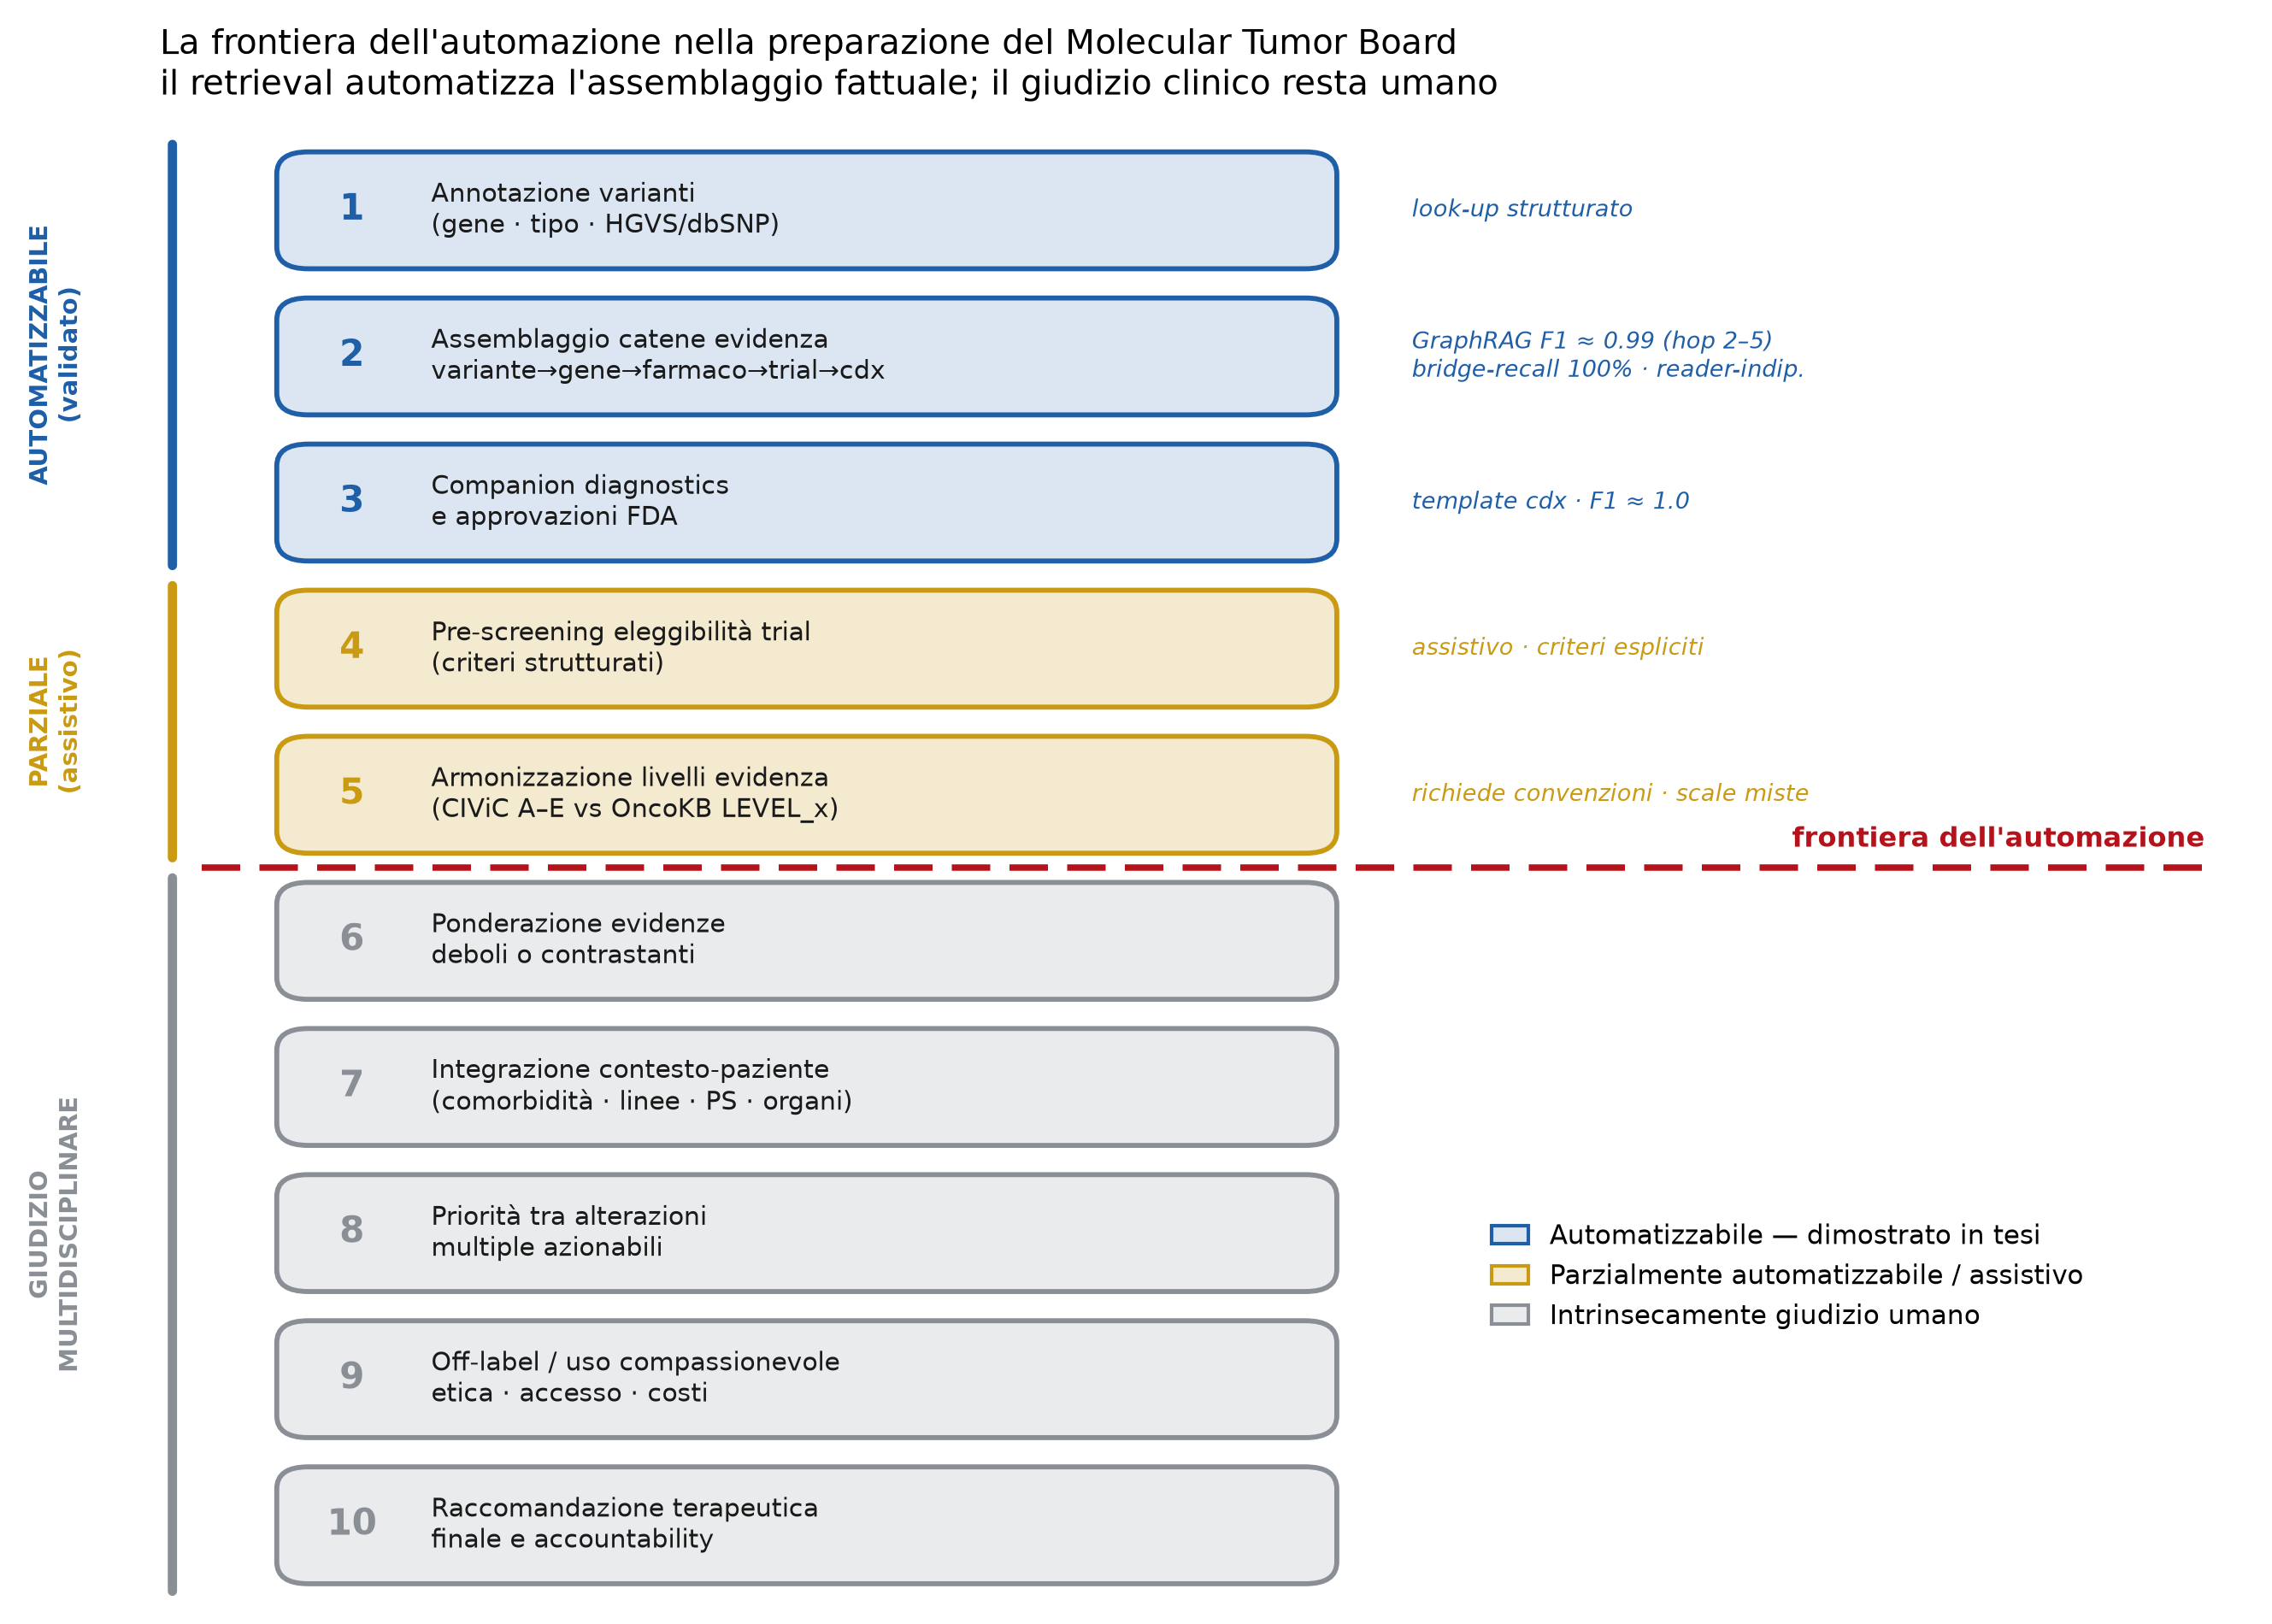
\includegraphics[width=0.98\textwidth]{fig9_automation_frontier.png}
\caption{La frontiera dell'automazione nella preparazione del Molecular
Tumor Board. I dieci stadi sono mappati in tre zone; i numeri empirici
(F1, bridge-recall) sono agganciati agli stadi che il sistema automatizza.
La linea rossa marca il confine tra recupero fattuale e giudizio clinico.}
\label{fig:frontiera}
\end{figure}

\section{Sopra la frontiera: il lavoro fattuale è delegabile}

Gli stadi 1--3 sono esattamente la parte \emph{tediosa e soggetta a errore}
della preparazione: recuperare e incrociare decine di associazioni
variante--farmaco--evidenza--trial da fonti eterogenee (CIViC, DGIdb,
ClinicalTrials.gov, FDA). È il lavoro che oggi consuma le ore di un analista
o di un biologo molecolare.

I risultati mostrano che questo lavoro è dimostrabilmente delegabile. Il
GraphRAG risolve le catene di ragionamento con \textbf{F1 $\approx$ 0,99
fino a 5 hop}, recuperando il \textbf{100\% dei fatti-ponte} necessari, e lo
fa con circa \textbf{25 volte meno contesto} del RAG testuale. Il vantaggio
non è un artefatto del particolare modello di lettura: sostituendo
completamente il reader (da \texttt{gemma3:27b} a \texttt{qwen3-coder-next},
famiglie e addestramenti diversi) la gerarchia non si muove a nessuna
profondità di hop. Ed è robusto alla riformulazione: le stesse domande
espresse in linguaggio clinico naturale non degradano la capacità del grafo
di seguire il cammino corretto.

\section{La frontiera è sicura perché il sistema la conosce}

Il punto concettualmente più importante non è l'accuratezza, ma
l'\emph{astensione}. Un sistema che automatizza il recupero fattuale in
ambito clinico è difendibile solo se sa riconoscere \emph{quando non ha una
risposta}. È qui che la struttura del grafo offre una garanzia che il RAG
testuale non può dare: quando la catena di fatti richiesta non esiste, il
GraphRAG produce un \textbf{contesto vuoto in modo deterministico}, e con un
guardrail elementare risponde ``NON DETERMINABILE'' invece di confabulare.

Sul benchmark di sicurezza il GraphRAG raggiunge il \textbf{punto ideale}:
astensione perfetta (1,00) sulle domande-trappola, zero allucinazioni, e
nessuna perdita sui controlli legittimi. In altre parole, il sistema
\textbf{restituisce l'incertezza al board umano invece di mascherarla}. È
proprio questa proprietà a tenerlo dal lato giusto della frontiera: non
invade il territorio del giudizio spacciando congetture per fatti.

\section{Sotto la frontiera: il giudizio resta umano}

Gli stadi 6--10 non contengono ``fatti da recuperare'': contengono
\emph{valutazioni da pesare}. Un'evidenza di livello D su un trial di fase I
va bilanciata contro la tossicità attesa nel paziente specifico, le linee di
terapia già fallite, l'accesso effettivo al farmaco, il performance status,
le comorbidità. Nessuno di questi elementi è nel grafo --- e non per un
limite implementativo che una versione futura potrebbe colmare, ma perché
\textbf{sono giudizi contestuali e responsabilità professionali}, non
associazioni recuperabili da una banca dati.

Gli stadi 4 e 5 stanno sulla frontiera stessa: il pre-screening di
eleggibilità e l'armonizzazione dei livelli di evidenza sono
parzialmente automatizzabili come supporto, ma richiedono convenzioni
esplicite e restano soggetti a verifica umana --- come mostra lo stesso
dataset, in cui coesistono scale di evidenza eterogenee (CIViC A--E e
OncoKB \texttt{LEVEL\_x}) che nessuna regola puramente sintattica può
riconciliare senza una decisione di merito.

\section{Conclusione}

L'automazione non sposta il confine tra macchina e clinico \emph{lungo} il
workflow MTB; lo rende \textbf{esplicito e sicuro}. La preparazione fattuale
--- assemblaggio e cross-referencing dell'evidenza molecolare --- è
largamente automatizzabile con affidabilità e, soprattutto, con astensione
deterministica sui casi senza risposta. Il giudizio multidisciplinare ---
ponderazione, contestualizzazione al paziente, priorità, responsabilità ---
resta intrinsecamente umano.

Il valore di un sistema come questo non è dunque rispondere \emph{di più},
ma sapere \emph{dove smettere di rispondere}: consegnare al Molecular Tumor
Board un dossier fattuale verificato, tracciabile fino alle fonti curate, e
insieme i suoi limiti dichiarati. È il board, non il sistema, a prendere la
decisione terapeutica --- ed è esattamente così che deve essere.

\end{document}
